\documentclass[a4paper]{article}

\usepackage{times}
\usepackage{tikz}
\usepackage[margin=0cm]{geometry}
\usepackage{graphicx}
\usepackage{anyfontsize}
\usepackage{fancyhdr}
\usepackage{indentfirst}
\usepackage{amsmath}
\usepackage[spanish]{babel}
\usepackage[utf8]{inputenc}
\usepackage{titlesec}
\usepackage{enumitem}
\usepackage{caption}
\usepackage{booktabs}

\author{}
\date{}
\title{}

\begin{document}
\thispagestyle{empty}

\newcommand{\saltoPag}{\newpage \noindent \thispagestyle{fancy}}

\begin{tikzpicture}[remember picture, overlay]
    \pgftransformshift{\pgfpoint{0cm}{0cm}}
    \draw [line width=2pt](1cm,-1cm) -- (1cm,-27.7cm) -- (14cm, -27.7cm) -- (14cm, -1cm) -- (1cm, -1cm);
    \draw[line width=2pt] (15cm, -27.7cm) -- (19cm,-27.7cm) -- (19cm, -1cm) -- (15cm, -1cm) --  (15cm, -27.7cm);
    \node [line width=2pt] at (17cm, -3.5cm) {
\includegraphics[width=3cm]{../imagenes/utn.png}};
		\node [line width=2pt] at (7.5cm, -7.5cm) {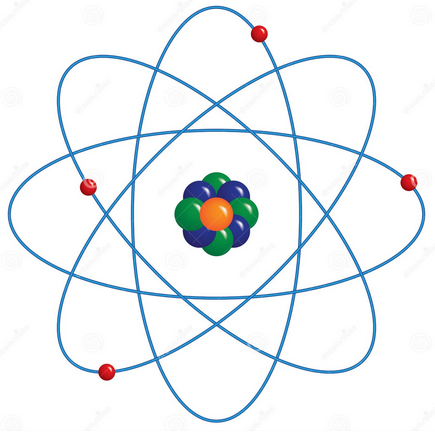
\includegraphics[width=6cm]{../imagenes/fotoAtomo.png}};
    \node at (17cm, -7cm) {\scalebox{5}{\textbf{U}}};
    \node at (17cm, -9cm) {\scalebox{5}{\textbf{T}}};
    \node at (17cm, -11cm) {\scalebox{5}{\textbf{N}}};
    \node at (17cm, -14cm) {\scalebox{5}{\textbf{F}}};
    \node at (17cm, -16cm) {\scalebox{5}{\textbf{R}}};
    \node at (17cm, -18cm) {\scalebox{5}{\textbf{C}}};
    \node at (7.5cm, -13cm) {\scalebox{2.5}{\textbf{Efecto Compton}}};

    \node at (7.5cm, -22cm) {
        \begin{minipage}[c]{12cm}
            \begin{itemize}
                \raggedright
                \vspace{1.5cm}
                \item \fontsize{12}{12}\selectfont \textbf{Autores:} \vspace {1mm} \fontsize{11}{12}\selectfont \\
                    \begin{itemize}
                        \item \hspace{2mm} Valentino Rao - Leg. 402308 \\
                        \item \hspace{2mm} Ignacio Ismael Perea - Leg. 406265 \\
                        \item \hspace{2mm} Manuel Leon Parfait - Leg. 406599 \\ 
                        \item \hspace{2mm} Gonzalo Filsinger - Leg. 400460 \\ 
                        \item \hspace{2mm} Agustín Coronel - Leg. 402010 \\
                        \item \hspace{2mm} Marcos Raúl Gatica - Leg. 402006 \\
                        \item \hspace{2mm} Santiago Pannunzio - Leg. 402350 \\
                    \end{itemize}

                \item \fontsize{12}{12}\selectfont \textbf{Curso:} 2R1. \\
                \item \fontsize{12}{12}\selectfont \textbf{Asignatura:} Física electrónica. \\
                \item \fontsize{12}{12}\selectfont \textbf{Institución:} Universidad Tecnológica Nacional - Facultad Regional de Córdoba \\

            \end{itemize}
        \end{minipage}};

\end{tikzpicture}

\renewcommand{\normalsize}{\fontsize{12}{18}\selectfont}
\newgeometry{margin=1cm} %Quiero dejar esto cercano a las normas APA,Rao: yo no quiero que se vea tan apretado, se queda a 1 cm, despues cambialo si queres
\fancyhf{}
\renewcommand{\headrulewidth}{0pt}
\renewcommand{\footrulewidth}{0.4pt}
\fancyfoot[R]{[Rao V. - Parfait M. - Filsinger G. - Perea I. - Coronel A - Pannunzio S. - Gatica M.] [\textbf{pág. \thepage}]}
\setlength{\footskip}{0pt}
\newpage
\thispagestyle{empty}
\text{}

\titleformat{\section} {\fontsize{12}{12}\bfseries}{\thesection.}{0.5em}{\underline}

\newpage
\newpage

\thispagestyle{empty}
\setcounter{page}{0}
\tableofcontents

\saltoPag
\twocolumn
\flushbottom
\section{INTRODUCCIÓN}

    \indent El siguiente informe busca detallar las prácticas de laboratorio para determinar:
    
    \begin{itemize}
        \item El valor de la mayor longitud de onda de la serie de Paschen.
        \item La longitud de onda de la línea espectral correspondiente a la transición del hidrógeno de estado n = 6 $\rightarrow$ 3.
        \item Longitud de onda de un fotón emitido por un átomo de hidrógeno al pasar de estado 10 al fundamental.
        \item Energía para extraer un electrón del átomo de hidrógeno en el estado n = 2.
        \item Diferencia de potencial necesaria para acelerar los electrones para que emita la primera línea de la serie de Balmer.
    \end{itemize}

\section{FUNDAMENTOS TEÓRICOS}
    \subsection{Modelo atómico de Thomson}
        \indent El modelo consiste en una masa de carga positiva sobre el cual quedan inmersas cargas negativas [ver figura a continuación]. Las demostraciones que fundamentaban este modelo del átomo no eran del todo adecuados debido al uso de los instrumentos de medición que se usaba. 

        \begin{figure}[h!]
            \centering
            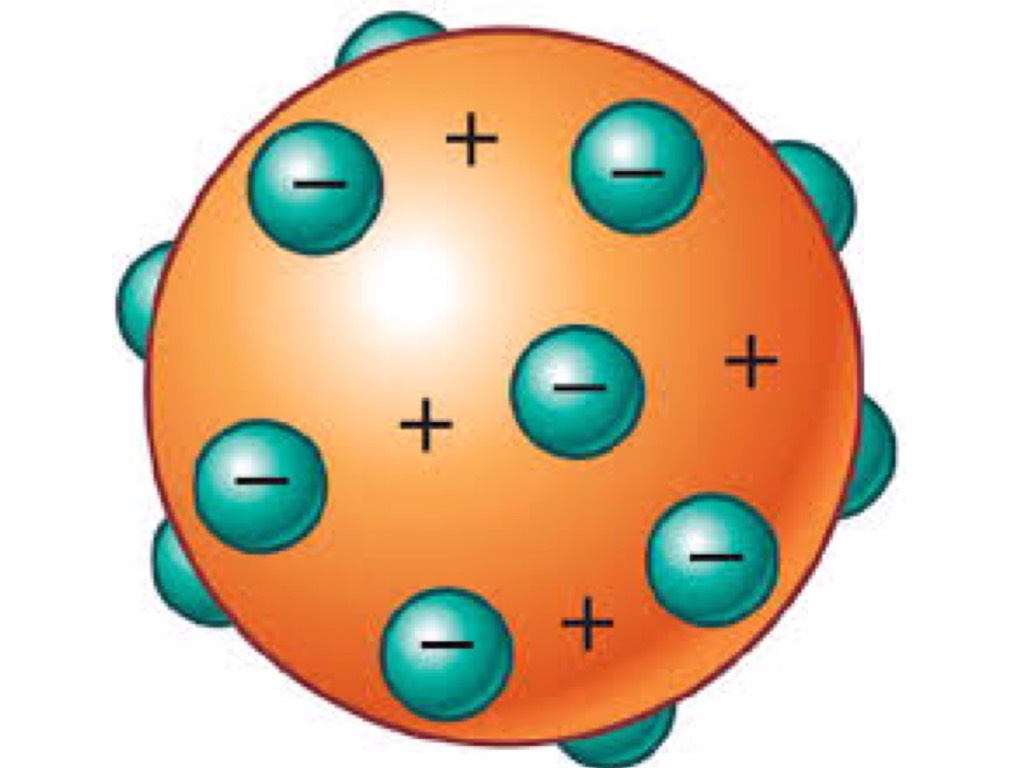
\includegraphics[width=4.5cm]{../imagenes/modeloAtomicoThomson.jpeg}
        \end{figure}

    \subsection{La excitación atómica}
        \indent Se sabe de dos mecanismos fundamentales capaces de excitar a un átomo:

        \renewcommand{\theenumi}{\roman{enumi}}
        \begin{enumerate}
            \item Provocando una interacción del átomo con otra partícula de tal forma que parte de la energía cinética sea absorbida por el átomo (como un choque o que un electrón pase cerca del núcleo atómico).
            \item Cuando un átomo recibe luz en cantidad suficiente para excitarlo.
        \end{enumerate}

        \indent Esto se asocia a darle energía de manera externa al átomo para que uno de sus electrones salte a un nivel de energía más alto (estado excitado). En ese punto, el átomo se vuelve inestable y buscará liberar la energía absorbida (haciéndolo en forma de fotones) para regresar a su estado más estable.
        \indent El o los fotones emitidos producen una línea espectral característica de la energía emitida (base de espectros de emisión).

    \subsection{Espectros atómicos}
        \indent Consiste en el análisis de la longitud de onda de una fuente luminosa. Hay cuatro tipos de clases de espectros:
        \begin{enumerate}
            \item Continuos de emisión.
            \item De líneas de emisión.
            \item Continuos de absorción.
            \item De líneas de absorción.
        \end{enumerate}

        \textbf{I - Continuos de emisión} \\
            \indent Es aquel que ocurre en sólidos a altas temperaturas, como un filamento de tungsteno o wolframio de una lámpara eléctrica.

            \begin{figure}[h!]
                \centering
                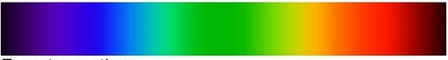
\includegraphics[width=4.5cm]{../imagenes/espectroContinuoDeEmision.png}
            \end{figure}

        \textbf{II - De líneas de emisión} \\
            \indent Se produce por descargas eléctricas en vapor de gas a altas temperaturas.
            \indent Los espectros de emisión se caracterizan por tener líneas claras sobre un fondo oscuro.

            \begin{figure}[h!]
                \centering
                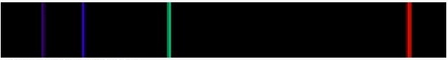
\includegraphics[width=4.5cm]{../imagenes/espectroLineasDeEmision.png}
            \end{figure}

        \textbf{III - Continuos de absorción}
            \indent Ocurre al hacer pasar un espectro continuo de emisión a través de un material de estado líquido o sólido. Se puede ver una franja con colores faltantes, aquellos que fueron absorbidos por el material en cuestión.

            \begin{figure}[h!]
                \centering
                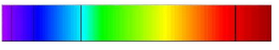
\includegraphics[width=4.5cm]{../imagenes/espectroContinuoDeAbsorcion.png}
            \end{figure}

        \textbf{IV - De líneas de absorción}
            \indent Ocurre cuando la luz pasa por un gas o vapor, el cual absorve algunas de las energías incidentes.

    \subsection{Series espectrales}

        \indent Son un conjunto matemático que determinan el valor de las longitudes de onda presentes en un espectro atómico.

        \textbf{Series espectrales del hidrógeno} \\
            Antes de la formulación de un modelo atómico robusto, los científicos determinaron experimentalmente un conjunto de series espectrales: \\

            \textit{Nota: para todos los casos, R es la constante de Raydberg y es igual a} $1,097 . 10^7 \frac{1}{m}$ \\

            \saltoPag

            \begin{itemize}
                \item \textbf{Serie de Lyman:} funciona para la emisión ultra violeta del hidrógeno, o sea, a altas frecuencias. 
                    \begin{center}
                        $\frac {1}{\lambda} = R(1 - {\frac{1}{n^2}})$ \hspace{2mm} $[n = 2,3,4,...]$
                    \end{center}

                \item \textbf{Serie de Balmer:} funciona para la emisión en el espectro visible.
                    \begin{center}
                        $\frac {1}{\lambda} = R({\frac{1}{2^2}} - {\frac{1}{n^2}})$ \hspace{2mm} $[n = 3,4,5,...]$
                    \end{center}

                \item \textbf{Serie de Paschem:} funciona para la emisión ultra violeta del hidrógeno a altas frecuencias.
                    \begin{center}
                        $\frac {1}{\lambda} = R({\frac{1}{3^2}} - {\frac{1}{n^2}})$ \hspace{2mm} $[n = 4,5,6,...]$
                    \end{center}

                \item \textbf{Serie de Brackett:} funciona para la emisión infrarroja, en bajas frecuencias.
                    \begin{center}
                        $\frac {1}{\lambda} = R({\frac{1}{4^2}} - {\frac{1}{n^2}})$ \hspace{2mm} $[n = 5,6,7,...]$
                    \end{center}

                \item \textbf{Serie de Pfund:} funciona para la emisión infrarroja.
                    \begin{center}
                        $\frac {1}{\lambda} = R({\frac{1}{5^2}} - {\frac{1}{n^2}})$ \hspace{2mm} $[n = 6,7,8,...]$
                    \end{center}
            \end{itemize}

    \newpage
    \noindent
    \thispagestyle{fancy}
        
    \section{Experiencia de laboratorio}

    \indent En el labotario hicimos una aproximaión al afecto compton, en el cual se observa la dispersión de fotones al chocar con un electrón. Para ello, se utilizaron los siguientes materiales:\\

    \begin{itemize}
        \item Pastilla radiactiva de bario-133.
        \item Pastilla radiactiva de Cadmio-109.
        \item Pastilla radiactiva de Cesio-137.
        \item Pastilla radiactiva de Cobalto-57.
        \item Pastilla radiactiva de Cobalto-60.
        \item Pastilla radiactiva de Manganeso-54.
        \item Pastilla radiactiva de Sodio-22.
        \item Pastilla radiactiva de Zinc-65.
        \item Detector de Geiger.
        \item Difusor de Plomo.
        \item Cilindro de Aluminio.
        \item Disco de Aluminio.
        \item 2 Discos de Plomo.
        \item Base de hierro.
    \end{itemize}

    \begin{figure}[h!]
        \centering
        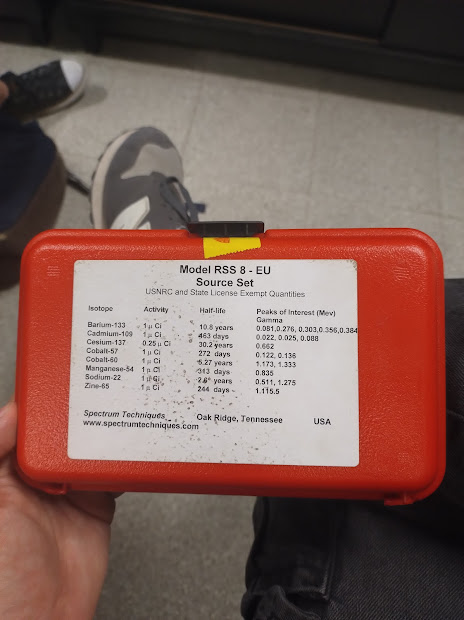
\includegraphics[width=4cm, trim={0cm 1cm 0cm 2cm}, clip]{../imagenes/pastillasrad.jpg}
        \caption{Pastillas radioactivas}
    \end{figure}


    \indent En el efecto comtpon cuando un material, en este caso las 8 pastillas radiactivas, emiten fotones, estos pueden ser dispersados por un electrón. La dispersión de los fotones se puede observar en un detector de Geiger, el cual se encarga de medir la cantidad de fotones que llegan a él, esto es posible ya que sabemos de manera matemático que este efecto se describe por la siguiente fórmula:\\

    \begin{center}
        \begin{equation}
            \lambda' - \lambda = \frac{h}{m_e c} (1 - cos(\theta))
        \end{equation}
    \end{center}

    \indent Donde $\lambda$ es la longitud de onda del fotón incidente, $\lambda'$ es la longitud de onda del fotón dispersado, h es la constante de Planck, $m_e$ es la masa del electrón, c es la velocidad de la luz y $\theta$ es el ángulo de dispersión, la fracción : $h \cdot (m_e \cdot c)^{-1}$ es conocida como longitud de onda de Compton, esta es una constante que vale $2.43 \cdot 10^{-12}$m $0.0243$Å y se representa como $\lambda_c$. Entonces la fórmula (1) se puede reescribir como:\\

    \begin{center}
        \begin{equation}
            \lambda' - \lambda =  \lambda_c \cdot (1 - cos(\theta))
        \end{equation}
    \end{center}

    \indent En el laboratorio hicimos una aproximación al efecto Compton, donde usamos 6 configuraciones en la que variamos como organizamos los discos de plomo y aluminio, el cilindro de plomo y aluminio. En cada configuración se midió la cantidad de fotones que llegaban al detector de Geiger cada 5 minutos.\\

    \begin{figure}[h!]
        \centering
        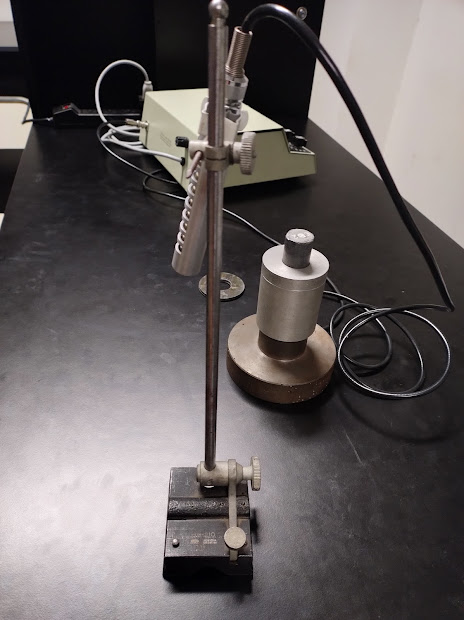
\includegraphics[width=4cm]{../imagenes/labcomton.jpg}
        \caption{Montaje experimental}
    \end{figure}
    
    \subsection{Mediciones}

    \indent A continuación se presentan los resultados obtenidos en el laboratorio:\\

    \begin{center}
        \begin{minipage}[c]{7.5cm}
            \centering
            \textbf{Tabla 1: Resultados de la experiencia de laboratorio}
            \vspace{2mm}
        \end{minipage}


        \begin{tabular}{ c c c c }
            \toprule
            N\textdegree Intentos & Voltaje (V) & Tiempo (s) & Radiación (CPM) \\
            \midrule
            1 & 1000 & 300 & 130 \\
            2 & 1000 & 300 & 134 \\
            3 & 1000 & 300 & 140 \\
            4 & 1000 & 300 & 124 \\
            5 & 1000 & 300 & 122 \\
            6 & 1000 & 300 & 132 \\
            \bottomrule
        \end{tabular}
    \end{center}

    \indent En la tabla 1 se observa la cantidad de fotones que llegaron al detector de Geiger en cada intento, vamos a detallar estos resultados:\\

    \indent La configuracion en el primer intento era de solo la base con las pastillas adentro y el contador, el resultado de 130 CPM se debe a que la base de hierro no es un material que pueda dispersar los fotones, por lo que la cantidad de fotones que llegaron al detector fue la misma que la cantidad de fotones emitidos por las pastillas.\\

    \begin{figure}[h!]
        \centering
        \vspace{-2mm}
        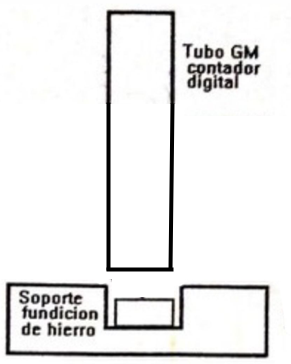
\includegraphics[width=2.5cm]{../imagenes/imagen1.png}
        \vspace{-5mm}
    \end{figure}

    \begin{center}
        \textbf{Configuración 1}\\
    \end{center}


    \newpage
    \noindent
    \thispagestyle{fancy}

    \indent En el segundo intento se colocó el difusor de plomo en la base de hierro y un cilindro de aluminio, el resultado de 134 CPM se debe a que el difusor de plomo es un material que puede dispersar los fotones, el aluminio absorve estos fotones y se produce el efecto Compton, por eso la cantidad de fotones que llegaron al detector fue ligeramente mayor que en el primer intento, ademas que en el primer intento no se midió 5 minutos exactos si no que se midió un minuto y se multiplicó por 5.\\

    \begin{figure}[h!]
        \centering
        \vspace{-2mm}
        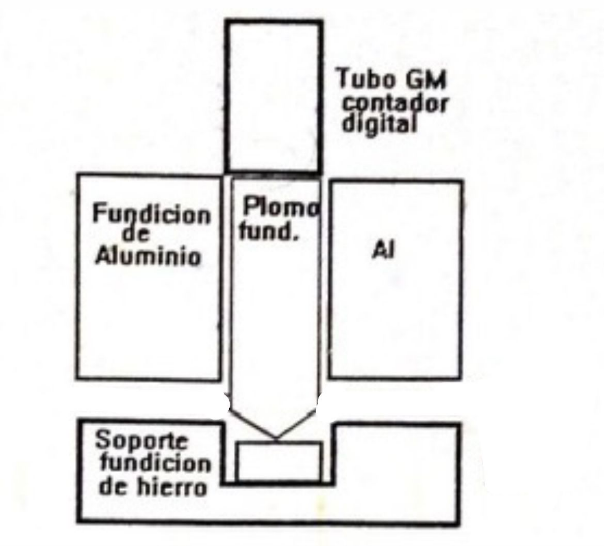
\includegraphics[width=4cm]{../imagenes/imagen2.png}
        \vspace{-5mm}
    \end{figure}

    \begin{center}
        \textbf{Configuración 2}\\
    \end{center}


    \indent En el tercer intento se colocó el difusor de plomo en la base de hierro y un disco de plomo debajo del cilindro de aluminio, el resultado de 140 CPM se debe a que el plomo es un material que puede dispersar los fotones, el aluminio absorve estos fotones y se produce el efecto Compton, por eso la cantidad de fotones que llegaron al detector fue mayor que en el segundo intento.\\

    \begin{figure}[h!]
        \centering
        \vspace{-2mm}
        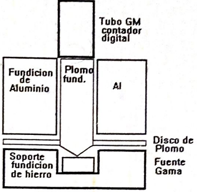
\includegraphics[width=3cm]{../imagenes/imagen3a.png}
        \vspace{-5mm}
    \end{figure}

    \begin{center}
        \textbf{Configuración 3}\\
    \end{center}

    \begin{figure}[h!]
        \centering
        \vspace{-2mm}
        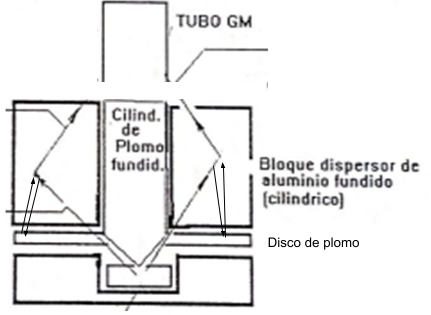
\includegraphics[width=4cm]{../imagenes/imagen3b.png}
        \vspace{-5mm}
    \end{figure}

    \begin{center}
        \textbf{Diagrama de rayos}\\
    \end{center}


    \indent En el cuarto intento se colocó el difusor de plomo en la base de hierro y un disco de plomo arriba del cilindro de aluminio, el resultado de 124 CPM concuerda con lo que decimos en la teoria, el difusor de plomo absorve los fotones en su dirreción y deja escapar algunos debido a su geometria, luego el aluminio absorve estos fotones, pero al tener un disco de plomo arriba del aluminio, este absorve los fotones que el aluminio no pudo absorver, por eso la cantidad de fotones que llegaron al detector fue menor que en el tercer intento.\\

    \begin{figure}[h!]
        \centering
        \vspace{-3mm}
        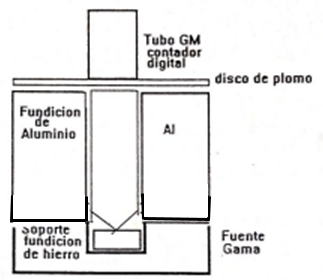
\includegraphics[width=4cm]{../imagenes/imagen4.png}
        \vspace{-5mm}
    \end{figure}

    \begin{center}
        \textbf{Configuración 4}\\
    \end{center}

    \newpage
    \noindent
    \thispagestyle{fancy}

    \indent En el quinto intento se colocó el difusor de plomo en la base de hierro y dos discos de plomo arriba del cilindro de aluminio, el resultado de 122 CPM concuerda con la configuración anterior, al tener otro disco de plomo arriba del aluminio, este absorve los fotones que el aluminio no pudo absorver, por eso la cantidad de fotones que llegaron al detector fue menor que en el cuarto intento.\\

    \begin{figure}[h!]
        \centering
        \vspace{-2mm}
        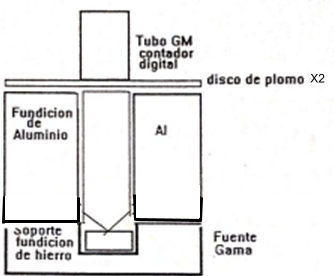
\includegraphics[width=4cm]{../imagenes/imagen5.png}
        \vspace{-5mm}
    \end{figure}

    \begin{center}
        \textbf{Configuración 5}\\
    \end{center}

    \indent En el sexto intento se colocó el difusor de plomo en la base de hierro, dos discos de plomo arriba del cilindro de aluminio y otro disco (grueso) de aluminio debajo del cilindro de aluminio, el resultado de 132 CPM  se debe a que los fotones que no absorve el difusor de hierro, son absorbidos por el aluminio, pero al tener un disco de aluminio debajo del cilindro de aluminio, se produce mas efecto compton, que no puede ser absorvido en su totalidad por los discos de plomo, por eso la cantidad de fotones que llegaron al detector fue mayor que en el quinto intento.\\

    \begin{figure}[h!]
        \centering
        \vspace{-2mm}
        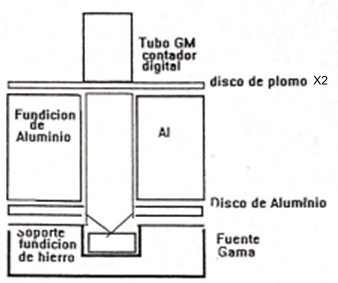
\includegraphics[width=4cm]{../imagenes/imagen6.png}
        \vspace{-5mm}
    \end{figure}

    \begin{center}
        \textbf{Configuración 6}\\
    \end{center}

    \section{CONCLUSIONES}

    \indent En la experiencia de laboratorio se pudo observar el efecto Compton, en el cual se observa la dispersión de fotones al chocar con un electrón. Se pudo observar que la cantidad de fotones que llegaron al detector de Geiger fue mayor en las configuraciones en las que se utilizó plomo, ya que este material es capaz de dispersar los fotones, mientras que el aluminio absorve estos fotones y se produce el efecto Compton.\\

\end{document}
